\documentclass[english,12pt]{article}
\usepackage{geometry}[margin=1in]
\usepackage{blindtext}
\usepackage{enumerate}
\usepackage{parskip} 
\usepackage{siunitx}
\usepackage{amsmath}
\usepackage{amsfonts}
\usepackage{amssymb}
\usepackage{hyperref}
\usepackage{listings}
\usepackage{inconsolata}
\usepackage{parskip}
\usepackage{graphicx}
\usepackage{wrapfig}
\usepackage{float}
\usepackage{listings}
\usepackage{xcolor}

\definecolor{codegreen}{rgb}{0,0.6,0}
\definecolor{codegray}{rgb}{0.5,0.5,0.5}
\definecolor{codepurple}{rgb}{0.58,0,0.82}
\definecolor{backcolour}{rgb}{0.90,0.92,0.95}

\lstdefinestyle{mystyle}{
    backgroundcolor=\color{backcolour},   
    commentstyle=\color{codegreen},
    keywordstyle=\color{magenta},
    numberstyle=\tiny\color{codegray},
    stringstyle=\color{codepurple},
    basicstyle=\ttfamily\footnotesize,
    breakatwhitespace=false,         
    breaklines=true,                 
    captionpos=b,                    
    keepspaces=true,                 
    numbers=none,                    
    numbersep=5pt,                  
    showspaces=false,                
    showstringspaces=false,
    showtabs=false,                  
    tabsize=2
}
\lstset{style=mystyle}

\graphicspath{./images}
\author{
    Cole Johnson - \texttt{cole.johnson@student.nmt.edu}
}
\title{
    \textbf{CSE326: Software Engineering} \\
    \LARGE{Assignment 2 - Design Patterns and OOD}
}
\begin{document}
 \maketitle
 \section*{Problem-Solving}
 \frenchspacing
 \begin{enumerate}[\bf (1.)]
  \item You are designing a Time and Talent Survey website for a local church. 
  Suppose the administrator would like to be notified whenever a new survey is completed.
  What design pattern is suggested? Why did you choose 
  this design pattern? (15 points)

  The observer / subject-object pattern would be an ideal design pattern to choose for this problem.
  I choose this design pattern because it's an effective tool when you have two aspects of a
  system that are both dependent on the other. Here, the subject could potentially be the survey 
  itself and participants could act as observers. 

  \item You are developing a graphics editor, within which shape can be basic or complex. 
  An example of simple shape is a line object; an example of a complex shape 
  is a rectangle object. The rectangle object consists of four-line objects. 
  Because all shapes have many common operations and can be represented in the 
  hierarchy, you wish to treat all shapes uniformly.
  What design pattern is suggested? Why did you choose this design pattern? 
  (15 points)

 The composite pattern would be an ideal design pattern to choose for this problem.
 This design pattern is good when you want to represent part-whole hierarchies--components
 that are composed of simpler items. Line objects could be the leaf or node while
 larger shapes make up the composite.
 \end{enumerate}
\pagebreak
\section*{Stack Implementation}
The stack implementation just has two parts: an array and a pointer to the next
unoccupied address inside the array. To push, just use the pointer to assign a new
element and increment the pointer. To pop, get the value that is pointed to,
decrement the pointer, and return the value. We need some additional helper functions
not described in the interface, like \texttt{grow()} and \texttt{isFull()} to help 
us grow the stack when needed.
\begin{figure}[H]
   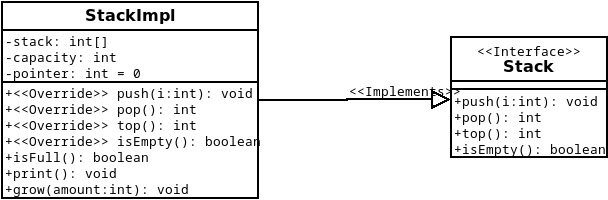
\includegraphics[width=10cm]{diagrams/StackImp.png}
\end{figure}
\section*{Decorator Pattern}
To make the decorators, I implemented an abstract class called \texttt{StackDecorator}.
The abstract class just holds a reference to the decorated stack, called \texttt{decoratedStack}.
Two concrete decorators, \texttt{StackDecorator1} and \texttt{StackDecorator2},
subclass the abstract decorator. Both the classes will call their specified behavior
and then just delegate the task of the task to \texttt{decoratedStack}.
\begin{figure}[H]
   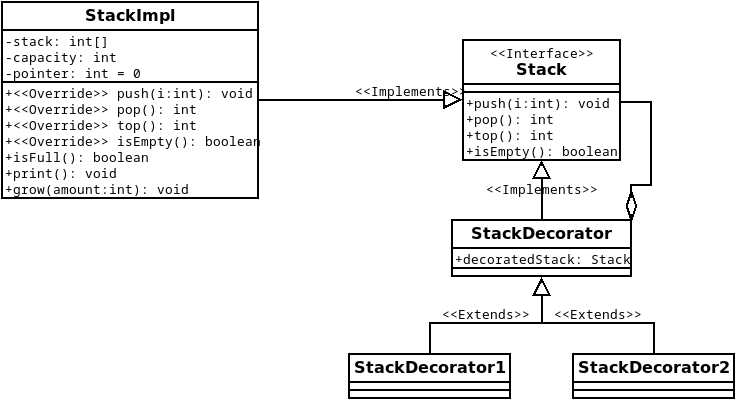
\includegraphics[width=10cm]{diagrams/StackDecorator.png}
\end{figure}
Here's the finally tested output using the driver code:
\begin{figure}[H]
   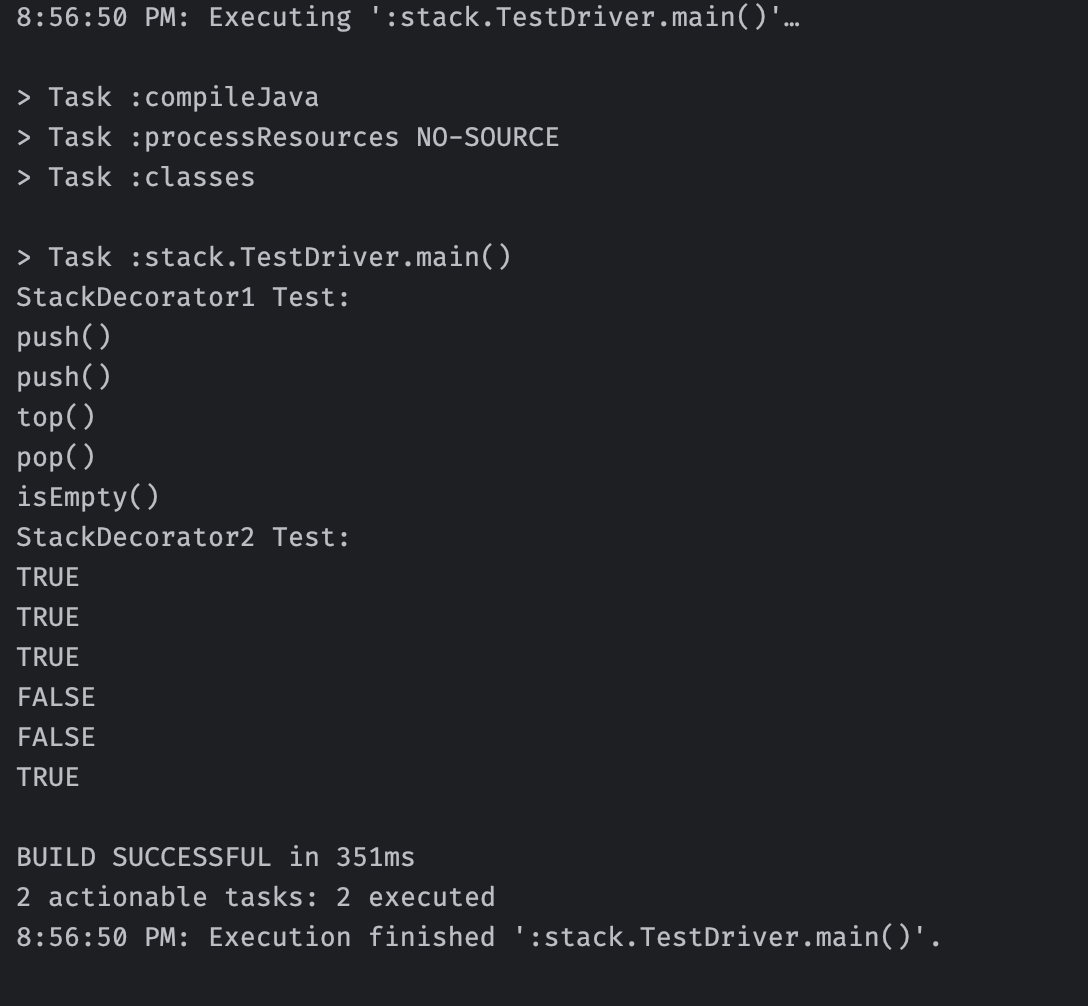
\includegraphics[width=10cm]{images/output.png}
\end{figure}
\end{document}  

